\documentclass[12pt]{article}

% packages
\usepackage{hyperref}
\hypersetup{
    colorlinks,
    citecolor=black,
    filecolor=black,
    linkcolor=black,
    urlcolor=blue
}

\usepackage{siunitx}

\usepackage{amsmath}

\usepackage{tikz}
\usetikzlibrary{circuits.ee.IEC}
\usepackage[siunitx, RPvoltages, american]{circuitikz}
\usetikzlibrary{calc}

\usepackage[danish]{babel}

% formatting
\setlength\parindent{0pt}

% command definitions
\newcommand{\lov}[2]{{\bf #1}\par\nobreak #2\vskip 5pt}
\newcommand{\regel}[2]{{\it #1} #2\vskip 5pt}
\newcommand{\enhed}[4]{{\bf #1} $\unit{#2}$\par\nopagebreak #3\par\nopagebreak #4\vskip 5pt}
\newcommand{\koge}[1]{\subsection{#1}}

\newcommand\gnd{%
\ensuremath{\mathbin{\text{\begin{tikzpicture}[circuit ee IEC,yscale=0.6,xscale=0.5]
\draw (0,2ex) to (0,0) node[ground,rotate=-90,xshift=.65ex] {};
\end{tikzpicture}}}}%
}

\newcommand\cvsource{%
\begin{circuitikz}\ctikzset{bipoles/vsourceam/inner plus={\tiny $+$}}\ctikzset{bipoles/vsourceam/inner minus={\tiny $-$}} \draw (0,0) to[cvsource, bipoles/length=0.7cm, invert] +(1,0);\end{circuitikz}%
}

\newcommand\cisource{%
\begin{circuitikz} \draw (0,0) to[cisource, bipoles/length=0.7cm] +(1,0);\end{circuitikz}%
}

\newcommand\vsource{%
\begin{circuitikz}\ctikzset{bipoles/vsourceam/inner plus={\tiny $+$}}\ctikzset{bipoles/vsourceam/inner minus={\tiny $-$}} \draw (0,0) to[vsource, bipoles/length=0.7cm, invert] +(1,0);\end{circuitikz}%
}

\newcommand\isource{%
\begin{circuitikz} \draw (0,0) to[isource, bipoles/length=0.7cm] +(1,0);\end{circuitikz}%
}

\newcommand\slojfe[1][->]{%
\begin{circuitikz}[scale=.5] \draw[#1,thick] (0,0) .. controls (.25,.3) and (.75,.3) .. (1,0);\end{circuitikz}%
}

\newcommand\rboks[3][.7]{%
\begin{tikzpicture}%
    \draw[red,ultra thick] (0,0) rectangle node[black,align=left]{#2} (#3,#1);%
\end{tikzpicture}%
}

\newcommand\termeq{%
\begin{tikzpicture}[scale=.3]%
    \draw[->] (0,0) -- ++(0,2) -- ++(-1,0);%
\end{tikzpicture}%
}

\newcommand\bipole[1]{%
    \begin{circuitikz}[scale=.5]%
	\draw (0,0) to[#1,bipoles/length=0.6cm] (2,0);%
    \end{circuitikz}%
}

\newcommand\short{%
    \begin{circuitikz}[scale=.5]%
	\draw (0,0) to[short,*-*] (1.5,0);%
    \end{circuitikz}%
}

\newcommand\colorul[3][black]{\color{#2}\underline{\color{#1}#3}\color{#1}}

\def\changemargin#1#2{\list{}{\rightmargin#2\leftmargin#1}\item[]}
\let\endchangemargin=\endlist

\begin{document}

\title{Formelsamling til Elektroteknik}
\author{Mathias \O. Selander}
\date{\today}
\maketitle

\begin{abstract}
    En formelsamling med formler indenfor faget elektroteknik. \emph{Indholdsfortegnelse på næste side.}
    \vskip 10pt
    Formelsamlingen er opdelt i 4 dele:
    \begin{description}
	\item[Love og Regler] En liste over forskellige love som kan bruges til at udregne forskellige værdier.
	\item[Matematik] Forskellig matematik til brug af løsning af differentiale ligninger f.eks.
	\item[Komponenter] En samling af komponenter og informationer omkring dem.
	\item[Kogebøger] Stens Kogebøger skrevet direkte af.
    \end{description}
\end{abstract}
\pagebreak

\tableofcontents
\pagebreak

\section{Love og Regler}
\lov{Kirchoffs str\o mlov (KCL)}{$I_1+I_2+I_3=0$}

\lov{Kirchoffs sp\ae ndings lov (KVL)}{$V_1+V_2+V_3=0$}

\lov{Effekt for passiv komponent($+\rightarrow -$)}{$P=VI$}
\lov{Effekt for aktiv komponent ($+\leftarrow -$)}{$P=-VI$}

\lov{Ohms lov}{$V_R=RI_R$}

\subsection{Serieopstillinger}
\lov{Alle Strømme er ens}{$I_t=I_1=I_2$}
\lov{Spændinger adderes}{$V_t=V_1+V_2$}
\lov{Ækvivalent modstand}{$R_{eq}=R_1+R_2$}
\lov{Spændingsdeler}{$$V_{R1}=V_t\cdot{R_1\over R_1+R_2}$$ $$V_{R2}=V_t\cdot{R_2\over R_1+R_2}$$}
\lov{Specielt, hvis $R_1=R_2$ da gælder}{$V_{R1}=V_{R2}={V_t\over 2}$}

\subsection{Parallelopstilling}
\lov{Alle Spændinger er ens}{$V_t=V_1=V_2$}
\lov{Strømme adderes}{$I_t=I_1+I_2$}
\lov{Ækvivalent modstand}{${1\over R_{eq}}={1\over R_1}+{1\over R_2}$}
\subsubsection{Specielt for \emph{netop to} modstande}
\lov{Ækvivalent modstand}{$R_{eq}=\frac{R_1R_2}{R_1+R_2}$}
\lov{Specielt hvis $R_1=R_2$ da gælder}{$R_{eq}={R_1\over 2}={R_2\over 2}$}
\lov{3 modstande (?)}{$R_{eq}=\frac{R_1}{3}=\frac{R_2}{3}=\frac{R_3}{3}$}
\lov{Strømdeling}{$I_{R1}=I_t\cdot{R_2\over R_1+R_2}$\par\nopagebreak$I_{R2}=I_t\cdot{R_1\over R_1+R_2}$}
\lov{Specielt hvis $R_1=R_2$ da gælder}{$I_{R1}=I_{R2}={I_t\over2}$}

\subsection{Thevenin og Norton}
\lov{Thevenin spænding er lig open circuit}{$V_t=V_{oc}$}
\lov{Norton strømmen er lig short circuit}{$I_n=I_{sc}$}
\lov{Thevenin og Norton modstand}{$R_t=R_n=\frac{V_{oc}}{I_{sc}}=\frac{V_t}{I_n}$}
\lov{Hvis ingen styrede kilder}{$R_n=R_t=R_{eq}$\termeq}
\lov{Effekt på load}{$P_L=V_t^2\frac{R_L}{(R_t+R_L)^2}$}
\lov{Maks effekt}{$P_{max}=\frac{V_tI_n}4$}
\lov{}{$P_{max}=\frac{V_t^2}{4R_t}$}

\subsubsection{Kildetransformation}
\lov{}{$R_n=R_t$}
\lov{Strøm $\rightarrow$ spænding}{$V_t=I_n\cdot R_n$}
\lov{Spænding $\rightarrow$ strøm}{$I_n=\frac{V_t}{R_t}$}

\subsection{Boolsk Algebra}
\lov{1.}{$A+B=B+A\quad;\quad AB=BA$}

\lov{2.}{$A+(B+C)=(A+B)+C\quad;\quad A(BC)=(AB)C$}

\lov{3.}{$A(B+C)=AB+AC\quad;\quad(A+B)(C+D)=AC+AD+BC+BD$}

\regel{1.}{$A\cdot 0=0$}

\regel{2.}{$A\cdot 1=A$}

\regel{3.}{$A+0=A$}

\regel{4.}{$A+1=1$}

\regel{5.}{$A\cdot A=A$}

\regel{6.}{$A+A=A$}

\regel{7.}{$A\cdot\overline A=0$}
           
\regel{8.}{$A+\overline A=1$}
           
\regel{9.}{$\overline{\overline A}=A$}

\regel{10A.}{$A+\overline A\cdot B=A+B$}

\regel{10B.}{$\overline A+A\cdot B=\overline A+B$}

\lov{Demorgan 1.}{$\overline{A\cdot B}=\overline A+\overline B$}
\lov{Demorgan 2.}{$\overline{A+ B}=\overline A\cdot\overline B$}

\lov{Xor}{$A\oplus B=\overline A\cdot B+A\cdot\overline B$}
\lov{Xnor}{$\overline{A\oplus B}=\overline A\cdot \overline B+A\cdot B$}

\subsection{Digitale byggeblokke}
\lov{Talrum}{$[0;2^n-1]$}
\lov{Talrum (2's complement)}{$[-2^{n-1};2^{n-1}-1]$}

\subsection{Ikke lineæere komponenter}
\subsubsection{Dioder}
\lov{Strøm som funktion af spænding for diode}{$I_d=\frac{V_S-V_d}{R_d}$}
\subsubsection{Transistorer}
\lov{Strøm på basis}{$I_B=\frac{V_{BB}-V_{BE}}{R_B}$}
\lov{Strøm på kollektor}{$I_C=\frac{V_{CC}-V_{CE}}{R_C}$}

\section{Matematik}
$$
    f(x)=e^{ax}\,\Rightarrow\left\{
	\begin{array}{l}
	    f'(x)=a\cdot e^{ax}\\
	    \int f(x)\,dx=\frac1a\cdot e^{ax}\\
	    f(0)=1\\
	    f(x)\rightarrow0\ \text{for}\ x\rightarrow -\infty,a>0\\
	    f(x)\rightarrow0\ \text{for}\ x\rightarrow \infty,a<0\\
	\end{array}
    \right.
$$
\subsection{Panserformlen}
$$
\begin{array}{l}
    y'(t)+p(t)\cdot y(t)=q(t)\\
    \Updownarrow\\
    y(t)=e^{-P(t)}\cdot\int e^{P(t)}\cdot q(t)\,dt+ke^{-P(t)}
\end{array}
$$

hvor $k$ er en konstant og $P(t)$ er en stamfunktion til $p(t)$

\section{Komponenter}
\subsection{Lineære Komponenter, Leksikon}
\begin{changemargin}{-4cm}{0cm}
	
    \begin{tabular}{p{9.5em}|l|l|l}
    Type & Modstand ($R$) & Kondensator ($C$) & Spole ($L$) \\ \hline

    Symbol & \begin{circuitikz}\draw (0,0) to[R,v=$V_R$,f=$I_R$] (2.5,0);\end{circuitikz} & \begin{circuitikz}\draw (0,0) to[C,v=$V_C$,f=$I_C$] (2.5,0);\end{circuitikz} & \begin{circuitikz}\draw (0,0) to[L,v=$V_L$,f=$I_L$] (2.5,0);\end{circuitikz} \\
    Ligning & \rboks{$V_R=R\cdot I_R$}{2.2} & \rboks{$I_C=C\cdot\frac{dV_C}{dt}$}{2.7} & \rboks{$V_L=L\cdot\frac{dI_L}{dt}$}{2.7} \\
    Enhed & $[R]=\si{\frac VA}=\Omega$ & $[C]=\si{\frac CV}=\si{\frac{AS}{V}}=$\rboks{$\si{s\cdot\Omega^{-1}}=\si{F}$}{2.2} & $[L]=\si{\frac{Vs}{A}}=$\rboks{$\si{s\Omega}=\si{H}$}{1.8} \\ \hline

    Serie & $R_{eq}=R_1+R_2$ & $\frac1{C_{eq}}=\frac1{C_1}+\frac1{C_2}\Leftrightarrow C_{eq}=\frac{C_1C_2}{C_1+C_2}$ & $L_{eq}=L_1+L_2$ \\
    Parallel & $\frac1{R_{eq}}=\frac1{R_1}+\frac1{R_2}\Leftrightarrow R_{eq}=\frac{R_1R_2}{R_1+R_2}$ & $C_{eq}=C_1+C_2$ & $\frac1{L_{eq}}=\frac1{L_1}+\frac1{L_2}\Leftrightarrow L_{eq}=\frac{L_1L_2}{L_1+L_2}$ \\ \hline

    $P_{øjeblik}$ & $P_{ø}=V_R\cdot I_R=\frac{V_R^2}{R}=R\cdot I_R^2$ & $P_{ø}=V_C\cdot I_C=CV_C\frac{dV_C}{dt}$ & $P_{ø}=V_L\cdot I_L=L\cdot I_L\cdot\frac{dI_L}{dt}$ \\
    $P_{middel}$ \small{$\begin{pmatrix}\text{Sinus med amplitude}\\V_A\text{\ og\ }V_{RMS}=\frac{V_A}{\sqrt2}\end{pmatrix}$} & $\begin{array}{ll}P_m & =V_{RAS}\cdot I_{RMS}\\&=\frac{V_{RMS}^2}{R}=\frac{V_A^2}{2R}\end{array}$ & $P_m=0$ & $P_m=0$ \\ \hline

    Oplagret energi & $\omega=0$ & $\omega=\frac12 C\cdot V_C^2$ & $\omega=\frac12 L\cdot I_L^2$ \\
    Steady state model = ``efter lang tid'' & \begin{circuitikz}\draw (0,0) to[R,v=$V_R$,f=$I_R$] (2.5,0);\end{circuitikz} & \begin{circuitikz}\ctikzset{open voltage position={legacy}}\draw (0,0) to[short,-*] ++(.5,0) to[open,v=$V_C$] ++(1.5,0) to[short,*-] ++(.5,0);\end{circuitikz} & \begin{circuitikz}\draw (0,0) to[short,f_={$I_L$}] (2.5,0);\end{circuitikz} \\
    Kontinutitet & Ingen krav & $\begin{array}{c}V_C(t_-)=V_C(t_+)\\V_C\text{\ er kontinuert}\end{array}$ & $\begin{array}{c}I_L(t_-)=I_L(t_+)\\I_L\text{\ er kontinuert}\end{array}$ \\ \hline
\end{tabular}

\end{changemargin}

\subsection{Andre gates lavet af NAND}
\lov{Not}{$X=\overline{A\cdot A}=\overline{A}$}
\begin{circuitikz}
    \ctikzset{logic ports=ieee}
    \draw ++(0,0)node[left]{A} to[inline not] (2,0) node[above]{X} node[right=5pt](end){=};
    \draw ++($ (end) + (2.3,0) $) node[nand port](nand){};
    \draw ++($ (end) + (.5,0) $) node[above]{A} to[short,-*] ++(.5,0) node(junc)[inner sep=0pt]{};
    \draw (junc) |- (nand.in 1);
    \draw (junc) |- (nand.in 2);
    \draw ++(nand.out) -- +(.5,0) node[above]{X};
\end{circuitikz}
\vskip 10pt

\lov{And}{$X=\overline{\overline{A\cdot B}}=A\cdot B$}
\begin{circuitikz}
    \ctikzset{logic ports=ieee}
    \draw (0,0) node[and port](and){};
    \draw (and.in 1) node[left]{A};
    \draw (and.in 2) node[left]{B};
    \draw ++(and.out) -- +(.2,0) node[above]{X} node[right=5pt](end){=};

    \draw ($ (end) + (2,0) $) node[nand port](nand1){};
    \draw ++($ (nand1) + (2.5,0) $) node[nand port](nand2){};
    \draw ++(nand1.out) to[short,-*] +(.1,0) |- (nand2.in 1);
    \draw ++(nand1.out) to[short,-*] +(.1,0) |- (nand2.in 2);
    \draw (nand1.in 1) node[left]{A};
    \draw (nand1.in 2) node[left]{B};
    \draw ++(nand2.out) -- +(.2,0) node[above]{X};
\end{circuitikz}
\vskip 10pt

\lov{Or}{$X=\overline{\overline A\cdot \overline B}=\overline{\overline A}+\overline{\overline B}=A+B$}
\begin{circuitikz}
    \ctikzset{logic ports=ieee}
    \draw (0,0) node[or port](or){};
    \draw (or.in 1) node[left]{A};
    \draw (or.in 2) node[left]{B};
    \draw ++(or.out) -- +(.2,0) node[above]{X} node[right=5pt](end){=};
    
    \draw ++($ (end) + (2,.75) $) node[nand port](nand1){};
    \draw ++($ (end) + (2,-.75) $) node[nand port](nand2){};
    \draw ++(nand1.in 1) -| ++(-.25,-.275) to[short,*-] +(-.2,0) node[left,inner sep=0pt](A){A};
    \draw ++(nand1.in 2) -| ++(-.25,.275) to[short,*-] (A);
    \draw ++(nand2.in 1) -| ++(-.25,-.275) to[short,*-] +(-.2,0) node[left,inner sep=0pt](B){B};
    \draw ++(nand2.in 2) -| ++(-.25,.275) to[short,*-] (B);

    \draw ($ (end) + (4.5,0) $) node[nand port](nand3){};
    \draw (nand1.out) -| (nand3.in 1);
    \draw (nand2.out) -| (nand3.in 2);
    \draw ++(nand3.out) -- +(.2,0) node[above]{X};
\end{circuitikz}
\vskip 10pt

\subsection{Opamp koblinger}
    \textbf{Inverterende}
    \nopagebreak

	\begin{circuitikz}
	    \draw (0,0) node[op amp](A1){};
	    \draw ++(A1.-)
		-- ++(-1,0)
		to[R=$R_1$] ++(-2,0)
		to[vsource,l_=$V_{in}$, invert] ++(0,-2)
		-- ++(2.5,0) node[left](Vom){}
		to[short,*-] ++(0,1) -- (A1.+);
	    \draw ++(A1.out)
		-- ++(1.5,0)
		to[open, v=$V_o$] ++(0,-1.5)
		-- (Vom);
	    \draw ++(A1.out) ++(.2,0)
		to[short,*-] ++(0,1.5)
		to[R=$R_2$] ++(-3,0)
		to[short,-*] ++(0,-1);
	\end{circuitikz}
	\vskip 10pt
	    $V_o=-V_{in}\left(\frac{R_2}{R_1}\right)$

	    $A_V=-\frac{R_2}{R_1}$

	    $R_{in}=\frac{V_{in}}{I_{in}}=R_1$

	    $R_o=\frac{V_{o,oc}}{I_{o,sc}}=0$

	\vskip 20pt
    \textbf{Ikke Inverterende}
    \nopagebreak

	\begin{circuitikz}
	    \draw (0,0) node[op amp, yscale=-1](A1){};
	    \draw ++(A1.+)
		-- ++(-2,0)
		to[vsource,v_=$V_{in}$,invert] ++(0,-3.5)
		-- ++(1.5,0) node[left](Vom){}
		to[R=$R_1$,*-*] ++(0,1.5) node[left](R1){}
		|- (A1.-);
	    \draw ++(A1.out)
		to[short,-*] +(.2,0) node[left](Vo){}
		to[short] ++(1.5,0)
		to[open,v=$V_o$] ++(0,-3)
		to[short] (Vom);
	    \draw ++(R1)
		to[R=$R_2$] ++(3,0)
		-| (Vo.east);
	\end{circuitikz}
	\vskip 10pt
	    $V_o=V_{in}\left(1+\frac{R_2}{R_1}\right)$

	    $A_V=1+\frac{R_2}{R_1}$

	    $R_{in}=\frac{V_{in}}{I_{in}}=\infty$

	    $R_o=\frac{V_{o,oc}}{I_{o,sc}}=0$

	\vskip 20pt
    \textbf{Spændingsfølger}
    \nopagebreak

	\begin{circuitikz}
	    \draw (0,0) node[op amp,yscale=-1](A1){};
	    \draw ++(A1.+)
		-- ++(-2,0)
		to[open,v=$V_{in}$] ++(0,-2.5)
		-- ++(5,0)
		to[open,v>=$V_o$] ++(0,2)
		-- (A1.out);
	    \draw ++(A1.out) ++(.2,0)
		to[short,*-] ++(0,-1.5)
		-- ++(-3,0)
		|- (A1.-);
	\end{circuitikz}
	\vskip 10pt
	    $V_o=V_{in}$

	    $A_V=1$

	    $R_{in}=\infty$

	    $R_o=0$

	\vskip 20pt
    \textbf{Differens}
    \nopagebreak

	\begin{circuitikz}
	    \draw (0,0) node[op amp](A1){};
	    \draw ++(A1.-)
		-- ++(-1.5,0)
		to[R,l_={\colorul{green}{$R_1$}}] ++(-1.5,0)
		-- ++(-1,0)
		to[V_=$V_2$,invert] ++(0,-3)
		-- ++(2.2,0) node[left](V1){}
		-- ++(1.8,0) node[left](R4){}
		-- ++(3.5,0)
		to[open,v>=$V_o$] ++(0,2.5)
		-- (A1.out);
	    \draw ++(V1.east)
		to[V=$V_1$,*-] ++(0,2)
		to[R={\colorul{green}{$R_3$}}] (A1.+);
	    \draw (R4.east) to[R={\colorul{red}{$R_4$}},*-*] (A1.+);
	    \draw ++(A1.-)
		to[short,*-] ++(0,1)
		to[R={\colorul{red}{$R_2$}}] ++(2.4,0)
		to[short,-*] (A1.out);
	\end{circuitikz}
	\vskip 10pt
	    $V_o=\left(\frac{R_4(R_1+R_2)}{R_1(R_3+R_4)}\right)\cdot V_1-\left(\frac{R_2}{R_1}\right)\cdot V_2$
	\vskip 10pt

	Hvis $R_3=R_1$ og $R_4=R_2$ da gælder

	    $V_o=\left(\frac{R_2}{R_1}\right)(V_1-V_2)$
	\vskip 10pt

	Og hvis $R_1=R_2=R_3=R_4$ da gælder

	$V_o=V_1-V_2$
	\vskip 20pt

    \textbf{Inverterende sumkobling}

    \nopagebreak
    \begin{circuitikz}
	\draw (0,0) node[op amp](A1){};
	\draw ++(A1.-)
	    -- ++(-1.5,0)
	    to[R={\colorul{green}{$R_1$}}] ++(-2,0)
	    to[open,v=$V_1$] ++(0,-2)
	    -- ++(1.5,0) node(V2m){}
	    -- ++(2,0) node(g){}
	    -- ++(3,0)
	    to[open,v>=$V_o$] ++(0,1.5)
	    to[short,-*] (A1.out);
	\draw ++(V2m)
	    to[open,v>=$V_2$] ++(0,1)
	    to[R={\colorul{green}{$R_2$}}] ++(1.5,0)
	    to[short,-*] ++(0,1);
	\draw ++(g.center)
	    to[short,*-] ++(0,-.2) node[tlground]{};
	\draw (g.center) -- (A1.+);
	\draw ++(A1.-)
	    to[short,*-] ++(0,.75)
	    to[R=$R_3$] ++(2,0)
	    -| (A1.out);
    \end{circuitikz}
    \vskip 10pt
    $V_o=-\left(V_1\frac{R_3}{R_1}+V_2\frac{R_3}{R_2}\right)$

    Specielt, hvis $R_1=R_2$

    $V_o=-\frac{R_3}{R_1}\cdot(V_1+V_2)$
 
\subsection{Flip-Flops}
\subsubsection{T-type}
\begin{circuitikz}
    \draw node[flipflop T]{};
\end{circuitikz}

\rboks{$Q^*=T\oplus Q$}{2.5}

\begin{tabular}{c|c}
    $T$ & $Q^*$ \\ \hline
    $0$ & $Q$ \\
    $1$ & $\overline Q$
\end{tabular}

\subsubsection{SR-type}
\begin{circuitikz}
    \draw node[flipflop SR]{};
    \draw (-.84,0) node[clockwedge](wedge){};
    \draw ++(wedge.center) -- +(-.3,0);
\end{circuitikz}

\rboks{$Q^*=S+\overline R Q$}{3}

\begin{tabular}{c|c}
    $SR$ & $Q^*$ \\ \hline
    $00$ & $Q$ \\
    $01$ & $0$ \\
    $10$ & $1$ \\
    $11$ & {\color{red} FORBUDT}
\end{tabular}

\subsubsection{JK-type}
\begin{circuitikz}
    \draw node[flipflop JK]{};
\end{circuitikz}

\rboks{$Q^*=J\overline Q+\overline K Q$}{3}

\begin{tabular}{c|c}
    $JK$ & $Q^*$ \\ \hline
    $00$ & $Q$ \\
    $01$ & $0$ \\
    $10$ & $1$ \\
    $11$ & $\overline Q$
\end{tabular}

\subsubsection{D-type}
\begin{circuitikz}
    \draw node[flipflop D]{};
\end{circuitikz}

\rboks{$Q^*=D$}{1.5}

\begin{tabular}{c|c}
    $D$ & $Q^*$ \\ \hline
    $0$ & $0$ \\
    $1$ & $1$
\end{tabular}


\section{Kogeb\o ger}
\subsection{Kogebog for kredsløb (alle kogebøgers moder)}
\begin{enumerate}
    \item Forsyn \emph{alle} komponenter med et unikt navn, F.eks.\ $R_1,R_2,S1,\ldots$
    \item Forsyn \emph{alle} komponenter med en strømpil ($\rightarrow$) samt ``+'' og ``-''. \emph{Du} bestemmer selv, om du vælger strømpilen aktiv eller passiv for kilder, men du skal vælge passiv for modstande.
    \item Giv alle strømme og spændingsforskelle et unikt navn, F.eks.\ $V_{R1},I_{R1},V_{S1},I_{S1},\ldots$
    \item Benyt i selvalgt rækkefølge
	\begin{itemize}
	    \item Ohms lov for \emph{hver} modstand. $V_{R1}=R_1\cdot I_{R1}$ , $V_{R2}=R_2\cdot I_{R2}$
	    \item KCL for alle knudepunkter
	    \item KVL for alle masker
	\end{itemize}
\end{enumerate}


\subsection{Knudepunktsmetoden}
\begin{circuitikz}
    \draw[thick] (0,0) rectangle node[above=55pt]{\underline{Faktaboks}} (6,5);
	   \draw
	++(1,3.5) node[left]{$V_A$} to[short, *-] +(1,0)
	to[R=$R_X$, v=$V_X$, f^>=$I_X$] +(3,0)
	to[short, -*] +(4,0) node[right]{$V_B$};
    \draw +(3, 2) node{$V_X=V_A-V_B$};
    \draw +(3, 1) node{$I_X=\frac{V_A-V_B}{R_X}$};
\end{circuitikz}

\begin{enumerate}
    \setcounter{enumi}{-1}
    \item Vælg et referencepunkt, og marker det med \gnd
    \item Navngiv alle øvrige knudepunkter F.eks.\ $V_A,V_B,\ldots$
    \item For alle spændingskilder, opskriv en ligning af typen

    \begin{circuitikz}
	\draw (0.5, 0) rectangle node{$V_A-V_B=10\unit{V}$} (3.5, 1);
	\draw ++(0,2) node[left]{$V_A$} to[short, *-] +(1.5,0)
	    to[vsource, v=$10\unit{V}$, invert] +(2.5,0)
	    to[short, -*] +(4,0) node[right]{$V_B$};
	\draw ++(6, 0) rectangle node{$V_A-V_B=2\unit{\frac VV}\cdot V_X$} +(3.5, 1);
	\draw ++(5.5,2) node[left]{$V_A$} to[short, *-] +(1.5, 0)
	    to[cvsource, v=$2\unit{\frac VV}\cdot V_X$, invert] +(2.5, 0)
	    to[short, -*] +(4,0) node[right]{$V_B$};
    \end{circuitikz}
    \item For alle knudepunkter der ikke rører en \emph{spændingskilde}, opskriv en ligning af nedenstående type (dog ikke referencepunkt). Hvis en spændingskilde sidder mellem to navngivne knudepunkter, da laves \emph{en fælles} ligning

    \begin{circuitikz}
	\draw ++(0,1) node[left]{$V_B$} to[short, *-] ++(.5,0)
	    to[R=$R_1$] ++(1,0)
	    to[short, -*] ++(.5,0) node[above right]{$V_A$};
	\draw ++(2,1) -- ++(0,.5)
	    to[isource, l=$2\unit{A}$, invert] ++(0,1) -- ++(0,.5);
	\draw ++(2,1) -- ++(0,-.5)
	    to[R=$R_2$] ++(0,-1)
	    to[short, -*] ++(0,-.5) node[below left]{$V_C$};
	\draw ++(2,1) -- ++(.5,0)
	    to[cisource, l=$2\unit{\frac AV}\cdot V_y$] ++(2,0);
	\draw ++(5,.5) rectangle node{$\frac{V_A-V_B}{R_1}+\frac{V_A-V_C}{R_2}-2A+2\unit{\frac AV}\cdot V_y=0$} +(6.5,1.5);
    \end{circuitikz}
    \item For styrede kilder, opskriv et dutryk for styrespændingen/styrestrømmen (se faktaboks)
    \item løs ligningen, $V_A=\ldots,V_B=\ldots$ (brug gerne maple)
    \item Bestem de $V$\!, $I$\! eller $P$\!, du blev spurgt om (se faktaboksen). For strømme gennem spændingskilder benyttes KCL
\end{enumerate}


\subsection{Superposition}
\begin{circuitikz}
    \draw (0,0) rectangle node[above=60pt]{\underline{Faktaboks}} node[above=40pt]{Nulstilling af kilder} (6.5,6);
    \draw ++(1.5,1) -- ++(0,1) to[vsource={0V},l_={=}] ++(0,1) -- +(0,1);
    \draw ++(2.5,1) -- node[right]{og} +(0,3);
    \draw ++(4,1) -- ++(0,1) to[isource={0A}, l_={=}] ++(0,1) -- +(0,1);
    \draw ++(5,1) to[short, -*] ++(0,0.7) ++(0,1.6) to[short, *-] +(0,0.7);
    \draw (1.5,0) node[above]{Kortslutning};
    \draw (4.4,0) node[above]{Afbrydelse};
\end{circuitikz}
\begin{description}
    \item[Betingelser]
	\begin{itemize}
	    \item[]
	    \item Kredsløbet må kun bestå af \emph{lineære} komponenter (kilder, modstande, kondensatorer, spoler, operationsforstærkere,\ldots)
	    \item Hvis Kredsløbet indeholder styrede kilder, \cvsource eller \cisource, bliver metoden \emph{besværlig}. $\Rightarrow$ så lad vær'.
	\end{itemize}
    \item[Fremgangsmåde]
	\begin{enumerate}
	    \item[]
	    \item Nulstil alle kilder (se faktaboks)
	    \item Tænd for kilderne, en ad gangen, og bestem den V eller I (ikke~P!), du blev spurgt om.
	    \item Læg bidragene for de enkelte kilder sammen, og vær omhyggelig med fortegn.
	\end{enumerate}
\end{description}


\subsection{Maskemetoden}
\begin{circuitikz}
    \draw (0,0) rectangle node[above=40pt]{\underline{Faktaboks}} (4,4);
    \draw ++(.5,2.5) node[above]{$R_x$} to[R, v_=$V_x$] +(3,0) node[above left]{$\rightarrow I_x$};
    \draw[<-] ++(1.5,3) .. controls +(.5,-.1) .. +(1,0) node[above]{$I_B$};
    \draw[->] ++(1.5,1.5) .. controls +(.5,.1) .. +(1,0) node[right]{$I_A$};
    \draw (.3,1) node[right]{$I_X=I_A-I_B$};
    \draw (.2,.5) node[right]{$V_X=R_X(I_A-I_B)$};
\end{circuitikz}
\begin{enumerate}
    \item Tegn en sløjfe, \slojfe[->], i alle masker, og navngiv maskestrømmene, $I_A,I_B,\ldots$
    \item For alle \emph{strømkilder}, opskriv en ligning af typen:

	\begin{center}
	\begin{circuitikz}
	    \draw (0,0) rectangle node{$I_A-I_B=2A$} (2.5,.7);
	    \draw ++(0,2) to[isource] node[above]{$2\unit A$} +(2.5,0);
	    \draw[->] ++(.7,1.3) .. controls +(.25,.1) and +(-.25,.1) .. +(1,0) node[below]{$I_A$};
	    \draw[<-] ++(.7,2.7) .. controls +(.25,-.1) and +(-.25,-.1) .. +(1,0) node[above]{$I_B$};
	\end{circuitikz}
	\hspace{5em}
	\begin{circuitikz}
	    \draw (0,0) rectangle node{$I_A-I_B=3\unit{\frac AA}\cdot I_X$} (3.5,.7);
	    \draw ++(0,2) to[cisource] node[above]{$3\unit{\frac AA}\cdot I_X$} +(3.5,0);
	    \draw[->] ++(1.2,1.3) .. controls +(.25,.1) and +(-.25,.1) .. +(1,0) node[below]{$I_A$};
	    \draw[<-] ++(1.2,2.7) .. controls +(.25,-.1) and +(-.25,-.1) .. +(1,0) node[above]{$I_B$};
	\end{circuitikz}
	\end{center}
    \item For alle masker, der ikke indeholder en \emph{strømkilde}, opskriv en ligning af nedenstående type. Hvis en strømkilde sidder mellem to masker, laves \emph{en fælles} ligning uden om kilden.

	\hspace{-7em}\begin{circuitikz}
	    \draw (0,0) -- +(-.2,0) +(0,0) -- +(0,-.2) +(0,0)
		to[short, *-] ++(0,1) to[R=$R_1$] ++(0,1) to[short, -*] ++(0,1) -- +(-.2,0) +(0,0) -- +(0,.2) +(0,0)
		to[vsource, l_=$5V$] ++(3,0) to[cvsource, l_=$2\unit{\frac VV}\cdot V_X$, invert] ++(1,0) to[short, -*] ++(1,0) -- +(.2,0) +(0,0) -- +(0,.2) +(0,0)
		to[R=$R_2$] ++(0,-3) to[short, -*] ++(0,0) -- +(.2,0) +(0,0) -- +(0,-.2) +(0,0)
		to[R=$R_3$] ++(-5,0);
	    \draw[->,scale=.75] ++(2,1.5) .. controls +(0,0.555) and +(-0.555,0) .. ++(1,1)
		.. controls +(0.555,0) and +(0,0.555) .. ++(1,-1)
		.. controls +(0,-.555) and +(.555,0) .. ++(-1,-1) node[above]{$I_A$}; 
	    \draw[->] ++(1.7,-1) .. controls +(.75,.1) .. +(1.5,0) node[right]{$I_C$};
	    \draw[->] ++(6,.7) .. controls +(-.1,.75) .. +(0,1.5) node[right]{$I_B$};
	    \draw ++(6.5,1) rectangle node{$R_1(I_A-0)-5\unit{V}+2\unit{\frac VV}\cdot V_X+R_2(I_A-I_B)+R_3(I_A-I_C)=0$} +(11,.7);
	\end{circuitikz}
    \item For styrede kilder, opskriv et udtryk for styrestrømmen/styrespændingen (se faktaboksen)
    \item Løs ligningerne, $I_A=\ldots,I_B=\ldots,$ (brug gerne maple)
    \item Bestem de V,I eller P, du blev spurgt om (se faktaboksen) for spændingsforeskelle over strømkilder, benyttes KVL.
\end{enumerate}


\subsection{Thevenins Ækvivalent (fra diagram)}
For \emph{alle lineære} kredsløb
\begin{enumerate}
    \item Bestem \rboks{$V_t=V_{oc}$}{1.7} (udgangsspænding uden belastning)

	\begin{circuitikz}
	    \draw (0,0) rectangle node[align=center]{Lineært\\kredsløb} (2,1);
	    \draw ++(2,.1) -- +(1,0) to[open, v={\ }, l_={$V_t=V_{oc}$}] +(1,.8) -- +(0,.8);
	\end{circuitikz} (Benyt masker, \emph{knudepunkter},\ldots)
    \item Tegn nu en Kortslutning mellem terminalerne, og bestem \rboks{$I_n=I_{sc}$}{2} (Kortslutnings strømmen)

	\begin{circuitikz}
	    \draw (0,0) rectangle node[align=center]{Lineært\\kredsløb} (2,1);
	    \draw ++(2,.1) -- +(1,0) to[short, *-*, l_={$\downarrow I_n=I_{sc}$}] +(1,.8) -- +(0,.8);
	\end{circuitikz} (Benyt \emph{masker}, knudepunkter,\ldots)
	
	Du kan som udgangspunkt \emph{ikke} ``genbruge'' ligninger fra punkt 1, da Kredsløbet er ændret.
    \item beregn \rboks{$R_n=R_t=\frac{V_{oc}}{I_{sc}}=\frac{V_t}{I_n}$}{4} (Den indre modstand)
    \item Tegn det ækvivalente kredsløb
	
	\hspace{-5em}\begin{circuitikz}
	    \draw ++(0,0) to[vsource={$V_t$}] ++(0,2) -- ++(1,0)
		to[R={$R_t$}] ++(1,0) -- ++(1,0)
		to[open, v={\ }] ++(0,-2) -- (0,0);
	\end{circuitikz}
	\hfill og/eller \hfill
	\begin{circuitikz}
	    \draw ++(0,0) to[isource, l={$I_n$}] ++(0,2)
		to[short,-*] ++(1.5,0)
		to[R={$R_n$}] ++(0,-2) -- (0,0);
	    \draw ++(1.5,2) -- ++(1.5,0)
		to[open, v={\ }] ++(0,-2) -- (0,0);
	\end{circuitikz}
\end{enumerate}


\subsection{Genvejsmetoden (til thevenin, diagram)}
Kun for \emph{lineære} kredsløb \emph{uden} styrede kilder - \emph{men megasmart!}
\begin{enumerate}
    \item \rboks{$V_t=V_{oc}$}{2} \emph{eller} \rboks{$I_n=I_{sc}$}{2}

	\begin{center}
	\begin{circuitikz}
	    \draw (0,0) rectangle node[align=center]{Lineært\\kredsløb} (2,1);
	    \draw ++(2,.1) -- +(1,0) to[open, v={\ }, l_={$V_t=V_{oc}$}] +(1,.8) -- +(0,.8);
	\end{circuitikz}
	\hspace{3em}
	\begin{circuitikz}
	    \draw (0,0) rectangle node[align=center]{Lineært\\kredsløb} (2,1);
	    \draw ++(2,.1) -- +(1,0) to[short, *-*, l_={$\downarrow I_n=I_{sc}$}] +(1,.8) -- +(0,.8);
	\end{circuitikz}
	\end{center}
    \item Bestem den ækvivalente modstand \rboks[1]{$R_n=R_t=R_{eq}$\termeq}{3.2} set fra terminalerne, når alle kilder nulstilles
    \item Beregn: \rboks{$R_n=R_t=\frac{V_{oc}}{I_{sc}}=\frac{V_t}{I_n}$}{4}
\end{enumerate}


\subsection{Theveninækvivalent (fyisk kredsløb)}
\begin{circuitikz}
    \ctikzset{bipoles/vsourceam/inner plus={\tiny $+$}}
    \ctikzset{bipoles/vsourceam/inner minus={\tiny $-$}}
    \ctikzset{bipoles/length=0.7cm}

    % D
    \draw ++(1,0.2) to[vsource=$V_t$] ++(0,1)
    -- ++(.2,0) to[R, l_=$R_t$] ++(1,0) -- ++(.7,0)
    to[open, v={\ }, l^={$V_o$}] ++(0,-1) -- (1,0.2);
    \draw[dashed,brown] ++(.2,.1) rectangle +(2.2,1.3);
    \draw[red, ultra thick] ++(4,.2) rectangle node[black]{$V_t=V_o$} +(1.7,.7);
    \draw[dashed] ++(0,0) rectangle +(8,2) node[below left,xshift=-28]{D: Ubelastet, dvs. $R_L=\infty$ og $I_o=0$};

    % C
    \draw ++(1,2.2) to[vsource=$V_t$] ++(0,1)
    -- ++(.2,0) to[R] ++(1.2,0) to[short, f={\ }] ++(.7,0) node[above=-3]{$I_o$}
    to[R, v={$V_o$}] ++(0,-1) -- (1,2.2);
    \draw[dashed,brown] ++(.2,2.1) rectangle +(2.2,1.3);
    \draw[red, ultra thick] ++(4,2.2) rectangle node[black]{$V_o=V_t-R_t\cdot I_o$} +(3,.7);
    \draw[dashed] ++(0,2) rectangle +(8,2.2) node[below left,xshift=-45]{C: Vi måler $V_o$ og $I_o$ ($R_L$ ukendt)};

    % B
    \draw ++(1,4.4) to[vsource=$V_t$] ++(0,1)
    -- ++(.2,0) to[R, l_=$R_t$] ++(1.2,0) to[short, f={\ }] ++(.7,0) node[above=-3]{$I_o$}
    to[R, l^={$R_L$}] ++(0,-1) -- (1,4.4);
    \draw[dashed,brown] ++(.2,4.3) rectangle +(2.2,1.3);
    \draw[red, ultra thick] ++(4.3,4.4) rectangle node[black]{$I_o=\frac{V_t}{R_t+R_L}$} +(2.3,1);
    \draw[dashed] ++(0,4.2) rectangle +(8,2.2) node[below left,xshift=-73]{B: Vi kender $R_L$ og måler $I_o$};

    % A
    \draw ++(1,6.6) to[vsource=$V_t$] ++(0,1)
    -- ++(.2,0) to[R, l_=$R_t$] ++(1.2,0) to[short] ++(.7,0)
    to[R, l^={$R_L$}, v={$V_o$}] ++(0,-1) -- (1,6.6);
    \draw[dashed,brown] ++(.2,6.5) rectangle +(2.2,1.3);
    \draw[red, ultra thick] ++(4.3,6.6) rectangle node[black]{$V_o=V_t\frac{R_L}{R_t+R_L}$} +(2.5,1);
    \draw[dashed] ++(0,6.4) rectangle +(8,2.2) node[below left,xshift=-70]{A: Vi kender $R_L$ og \emph{måler} $V_o$};

    \draw (1,9) node{\underline{Faktaboks}};

\end{circuitikz}
\begin{enumerate}
    \item Tilslut en belastning (gerne $R_L=\infty$, ubelastet)
    \item Opskriv en ligning (se faktaboksen)
    \item Tilslut en \emph{ny} belastning
    \item Opskriv en \emph{ny} ligning (se faktaboksen)
    \item Løs ligningerne, og bestem derved $V_t$ og $R_t$
    \item Beregn:

	\begin{center}
	    \rboks{$I_n=\frac{V_t}{R_t}$}{2}

	    \rboks{$R_n=R_t$}{2}
	\end{center}
    \item Tegn det ækvivalente kredsløb
	
	\hspace{-5em}\begin{circuitikz}
	    \draw ++(0,0) to[vsource={$V_t$}] ++(0,2) -- ++(1,0)
		to[R={$R_t$}] ++(1,0) -- ++(1,0)
		to[open, v={\ }] ++(0,-2) -- (0,0);
	\end{circuitikz}
	\hfill og/eller \hfill
	\begin{circuitikz}
	    \draw ++(0,0) to[isource, l={$I_n$}] ++(0,2)
		to[short,-*] ++(1.5,0)
		to[R={$R_n$}] ++(0,-2) -- (0,0);
	    \draw ++(1.5,2) -- ++(1.5,0)
		to[open, v={\ }] ++(0,-2) -- (0,0);
	\end{circuitikz}
\end{enumerate}


\subsection{Operationsforstærker (Opamp)}
\begin{circuitikz}
    \draw (0,0) node[op amp](A1){};
    \draw ++(A1.-)
	to[short,f_<=$I_-$] ++(-3,0)
	-- ++(-1,0)
	to[open, v>=$V_d$] ++(0,-1)
	to[short,-*] ++(1,0) node[below right]{$V_+$}
	to[short,f_>=$I_+$] (A1.+);
    \draw ++(A1.-) ++(-3,0)
	to[short,*-,l_=$V_-$] ++(0,1)
	-- ++(3,0)
	to[R] ++(1,0)
	-| (A1.out);
    \draw ++(A1.out)
	to[short,*-] ++(1,0)
	to[open,v=$V_o$] ++(0,-1.5)
	-- ++(-6.4,0) node(gnd){}
	-- ++(-1,0);
    \draw ++(gnd)
	to[short,*-] ++(0,-.1) node[tlground]{};
    \draw[<-,brown,thick] ++(A1.out) ++(.3,.3) .. controls +(1.2,.7) .. +(2.5,1)
    node[right,align=left]{Ingen knudepunktsligning\\for dette punkt};
\end{circuitikz}
\begin{enumerate}
    \item Kontroller, at der sidder en \bipole{R}\ eller \short\ mellem udgangen og "$-$" indgangen. \emph{(Det gør der altid!)}
    \item Opskriv og benyt: \rboks[2]{%
		$I_+=0$ \\%
		$I_-=0$ \\%
		$V_d=0\Leftrightarrow V_+=V_-$%
	}{4}
    \item Gør som du plejer, altså
	\begin{enumerate}
	    \item Benyt skiftevis KVL, Ohms lov, KCL, Ohms lov, KVL fra venstre mod højre, og brestem alle ubekendte. Du er færdig, når du kan lave en KVL med $V_o$.
	    \item Benyt Knudepunktsmetoden, \emph{men}
		\begin{itemize}
		    \item Ingen ligning for punktet ved udgangen
		    \item Ny ligning: \rboks{$V_+=V_-$}{1.7}
		\end{itemize}
	\end{enumerate}
\end{enumerate}


\subsection{Tilstandsmaskiner}
\begin{changemargin}{-3.6cm}{0cm}
	
\parbox{.4in}{
    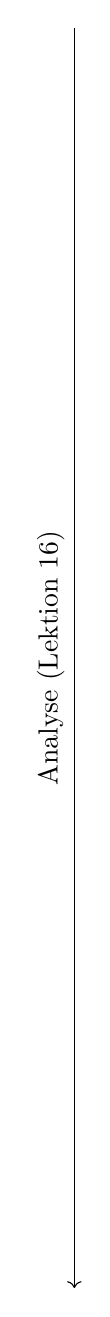
\begin{tikzpicture}
	\draw[<-] (0,0) -- node[rotate=90,above]{Analyse (Lektion 16)} (0,16);
    \end{tikzpicture}
}
\parbox{3in}{
    \begin{itemize}
	\item Karateristiske ligninger
	\item Exitationsligninger
	\item outputligninger
    \end{itemize}
    ---
    \begin{itemize}
	\item List alle kombinationer af $Q_n,\ldots,Q_0$
	\item Udfyld $Q^*$ Vha. ligningerne
	\item Udfyld output cha. ligningerne
    \end{itemize}
    ---
    \begin{itemize}
	\item Giv hver tilstand et navn
	\item Udfyld $T^*$
    \end{itemize}
    ---
    \begin{itemize}
	\item Tegn en ``Bolle'' for hver tilstand
	\item Tiføj pile og \colorul{red}{outputs}
    \end{itemize}
    ---
    \begin{itemize}
	\item Lav en række for $T$ vha. pilediagrammet
	\item Udfyld outputs
    \end{itemize}
}
\parbox{1.2in}{
    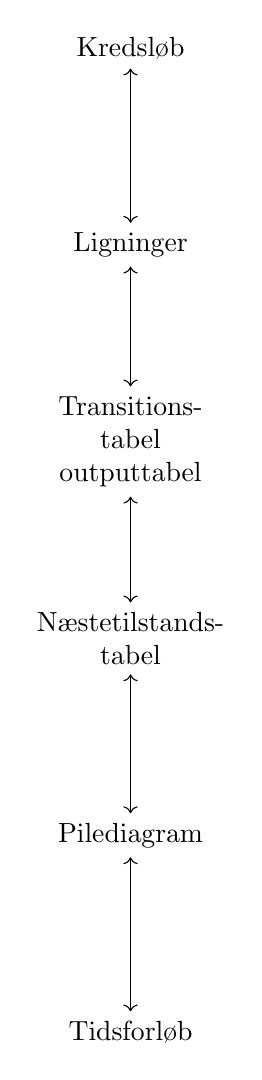
\begin{tikzpicture}
	\node at (0,0) (A) {Tidsforløb};
	\node at (0,2.5) (B) {Pilediagram};
	\node[align=center] at (0,5) (C) {Næstetilstands-\\tabel};
	\node[align=center] at (0,7.5) (D) {Transitions-\\tabel\\outputtabel};
	\node at (0,10) (E) {Ligninger};
	\node at (0,12.5) (F) {Kredsløb};
	\draw[<->] (A) -- (B);
	\draw[<->] (B) -- (C);
	\draw[<->] (C) -- (D);
	\draw[<->] (D) -- (E);
	\draw[<->] (E) -- (F);
    \end{tikzpicture}
}
\parbox{3in}{
    \begin{itemize}
	\item Tegn alle D-flip-Flops
	\item Husk synkron clk
	\item Tegn exitationslogik
	\item tegn outputlogik
	\item Selvkorrigerende
    \end{itemize}
    ---
    \begin{itemize}
	\item Bestem all $Q^*=D$ og outputs (evt.\ vha.\ k-kort) ``simple'' logiske kredsløb med $Q_n,\ldots,Q_0$ og brugerinputs som input. Nyt k-kort for \emph{hver} $Q^*=D$ og output.
    \end{itemize}
    ---
    \begin{itemize}
	\item Bestem antal D-flip-Flops
	\item Tildel en bitkombination til hver tilstand

	    Lad $Q^*$ være don't care for ubrugte Tilstandsmaskiner
	\item Tilføj outputs
    \end{itemize}
    ---
    \begin{itemize}
	\item Lav $T$ og $T^*$ søjlr vha.\ pilediagrammet
    \end{itemize}
    ---
    \begin{itemize}
	\item Bestem antallet af tilstande, og tegn pilediagrammet (se på sekvenslængden)
    \end{itemize}
}
\nolinebreak
\parbox{.5cm}{\ }
\nolinebreak
\parbox{.4in}{
    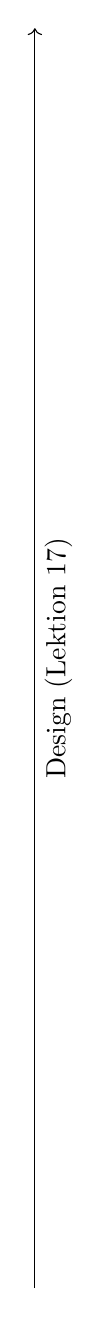
\begin{tikzpicture}
	\draw[->] (0,0) -- node[rotate=90,below]{Design (Lektion 17)} (0,16);
    \end{tikzpicture}
}

\end{changemargin}


\subsection{Dioder}
\begin{enumerate}
    \item Opskriv \rboks[.8]{$I_d=\frac{V_s-V_d}{R_d}$}{2.5}
    \item Vælg to ``tilfældige'' $V_d$-værdier
    \item Bestem $I_d(V_d)$ vha 1. for hver $V_d$-værdi
    \item Tegn linien og aflæs skæringspunktet
\end{enumerate}


\subsection{Diodemodeller}
\begin{enumerate}
    \item For hver diode: gæt ON eller OFF
    \item Indsæt \begin{circuitikz}
	    \draw ++(0,0) to[short,-*] ++(.5,0) to[open] ++(.5,0) to[short,*-] ++(.5,0);
	    \node at (0.3,0.2) {$+$};
	    \node at (.75,.25) {$V_d$};
	    \node at (1.2,0.2) {$-$};
    \end{circuitikz} for OFF eller \begin{circuitikz}
	\ctikzset{bipoles/vsourceam/inner plus={\tiny $+$}}
	\ctikzset{bipoles/vsourceam/inner minus={\tiny $-$}}
	\draw (0,0) to[vsource, bipoles/length=0.7cm, invert,l^=$V_k$] ++(1,0) to[short,f^=$I_d$] ++(.5,0);
    \end{circuitikz} for ON på diodens plads
\item Gør som du pljer, og bestem $V_d$ for OFF og $I_d$ for ON
\item Kontroller, at $V_d<V_k$ for OFF og $I_d>0$ for ON
\item \emph{ommer}, hvis 4. ikke er opfyldt!
\end{enumerate}


\subsection{Kondensator og Spole}
For \bipole{C} er $V_C(t)$ primær variabel

For \bipole{L} er $I_L(t)$ primær variabel

(pga.\ kontinuitet)

\begin{enumerate}
    \item Bestem startværdi (ud fra $t<0$) og slutværdi ($t\rightarrow\infty$) for primær varible ved hjælp af 2x steady state
    \item Bestem \rboks{$\tau=R_{eq}\cdot C$}{2.5} eller \rboks{$\tau=\frac{L}{R_{eq}}$}{1.5}, hvor $R_{eq}$ er den ækvivalente modstand, som $C$ eller $L$ ser ind i for $t\ge0$
    \item \ 

	\parbox{5em}{Opskriv:\vskip 4pt eller:}\parbox{40em}{\rboks[1.2]{$V_C(t)=V_{C,slut}+\left(V_{C,start}-V_{C,slut}\right)\cdot e^{-t/\tau}\ ,t\ge0$\\$I_L(t)=I_{L,slut}+\left(I_{L,start}-I_{L,slut}\right)\cdot e^{-t/\tau}\ ,t\ge0$}{9}}
    \item Bestem evt. andre $V$ eller $I$ for kredsløbet. Benyt f.eks.\ KVL, KCL, ohm $I_C=C\cdot\frac{dV_C}{dt}$ og/eller $V_L=L\cdot\frac{dI_L}{dt}$ 
\end{enumerate}


\subsection{Transistormodeller}
\begin{enumerate}
    \item Gæt transistorens tilstand
    \item Indsæt modellen og husk betingelser
    \item Gør som du plejer, og besktem de $I$ eller $V$, der indgår i modellens betingelser
    \item Kontroller, at alle betingelser er opfyldt
    \item \emph{Ommer}, hvis betingelserne ikke er \emph{ok}
\end{enumerate}

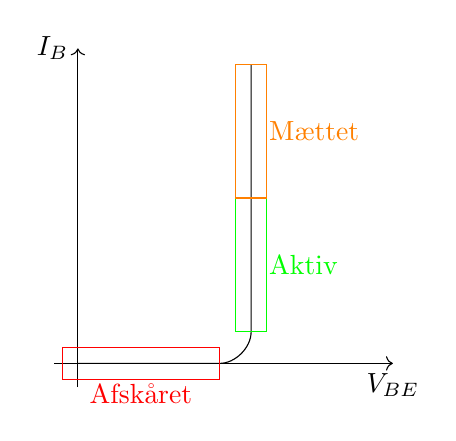
\begin{tikzpicture}
    \draw[->] (-.3,0) -- (4,0) node[below]{$V_{BE}$};
    \draw[->] (0,-.3) -- (0,4) node[left]{$I_B$};
    \draw (0,0) -- ++(1.8,0) node(afend){}
	.. controls ++(.2,0) and ++(0,-.2) .. ++(.4,.4) node(akbeg){}
	-- ++(0,1.7) node(akend){}
	-- ++(0,1.7) node(mend){};
    \draw[red] (-.2,-.2) rectangle node[below=4pt]{Afskåret} ($ (afend) + (0,.2) $);
    \draw[green] ($ (akbeg) + (-.2,0) $) rectangle node[right=3pt]{Aktiv} ($ (akend) + (.2,0) $);
    \draw[orange] ($ (akend) + (-.2,0) $) rectangle node[right=3pt]{Mættet} ($ (mend) + (.2,0) $);
\end{tikzpicture}
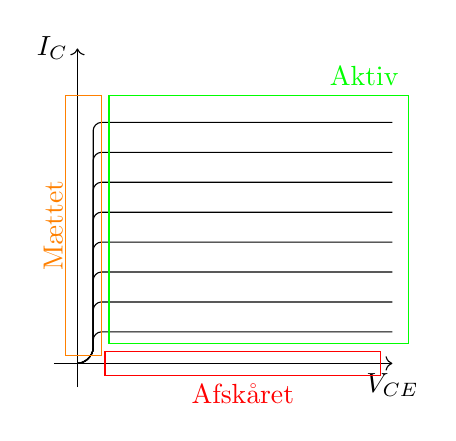
\begin{tikzpicture}
    \draw[->] (-.3,0) -- (4,0) node[below]{$V_{CE}$};
    \draw[->] (0,-.3) -- (0,4) node[left]{$I_C$};
    \foreach \y in {.4,.78,...,3.4}
	\draw ++(0,0) .. controls ++(.1,0) and ++(0,-.1) ..
	    ++(.2,.2) -- ++($ (0,\y) - (0,.3) $)
	    .. controls ++(0,.05) and ++(-.05,0) .. (.3,\y) -- (4,\y);
    \draw[orange] (-.15,.1) rectangle node[rotate=90,above=4pt]{Mættet} (.3,3.4);
    \draw[red] ++(.35,-.15) rectangle node[below=4pt]{Afskåret} ++(3.5,.3);
    \draw[green] ++(.4,.25) rectangle (4.2,3.4) node[above left]{Aktiv};
\end{tikzpicture}
\nopagebreak
\vskip 10pt
\nopagebreak
\hrule
\nopagebreak
\parbox{7em}{\color{red} Afskåret

(Cut-off)}
    \parbox{10em}{
\begin{circuitikz}
    \draw ++(1.25,0) node[left]{$-$} node[right]{$E$} to[short,-*] ++(0,0.75);
    \draw ++(0,1) node[left]{$B$} -- ++(.5,0) node(pB){} to[short,-*]  ++(.5,0);
    \draw (pB) node[above]{$+$};
    \draw (pB) node[below]{$+$};
    \draw ++(1.25,2) node[left]{$-$} node[right]{$C$} to[short,-*] ++(0,-.75);
    \draw (pB) node[above=10pt]{$V_{BC}$};
    \draw (pB) node[below=10pt]{$V_{BE}$};
\end{circuitikz}
}
\parbox{7em}{\color{blue} Betingelser:

    \hspace{5pt} $V_{BE}<0.5\si{V}$

    \hspace{5pt} $V_{BC}<0.5\si{V}$
}
\nopagebreak
\hrule
\nopagebreak
\parbox{7em}{\color{orange} Mættet 

(Saturated)}
    \parbox{10em}{
\begin{circuitikz}
    \ctikzset{bipoles/vsourceam/inner plus={\tiny $+$}}
    \ctikzset{bipoles/vsourceam/inner minus={\tiny $-$}}

    \draw ++(1.5,0) node[right]{$E$} to[short,-*] ++(0,.75) node[right](center){} to[vsource,v_={$0.2\si{V}$},f^<={$I_C$},bipoles/length=1cm] ++(0,1.75) node[right]{$C$};
    \draw ++(center) to[vsource,v^={$0.7\si{V}$},f_<={$I_B$},bipoles/length=1cm] ++(-2,0) node[below]{$B$};
\end{circuitikz}
}
\parbox{7em}{\color{blue} Betingelser:

    \hspace{5pt} $I_B>0$

    \hspace{5pt} $\beta\cdot I_B>I_C>0$
}
\nopagebreak
\hrule
\nopagebreak
\parbox{7em}{\color{green} Aktiv 

(Active)}
    \parbox{10em}{
\begin{circuitikz}
    \ctikzset{bipoles/vsourceam/inner plus={\tiny $+$}}
    \ctikzset{bipoles/vsourceam/inner minus={\tiny $-$}}

    \draw ++(1.5,0) node[right]{$E$} to[short,-*] ++(0,.75) node[right](center){} to[cisource,invert,bipoles/length=1cm] node[left]{$\beta\cdot I_{B}$} ++(0,1.75) node[right]{$C$};
    \draw ++(center) to[vsource,v^={$0.7\si{V}$},f_<={$I_B$},bipoles/length=1cm] ++(-2,0) node[below]{$B$};
    \node[align=left] at (2.3,.8) {$+$\\$V_{CE}$\\$-$};
\end{circuitikz}
}
\parbox{7em}{\color{blue} Betingelser:

    \hspace{5pt} $I_B>0$

    \hspace{5pt} $V_{CE}>0.2\si{V}$
}
\nopagebreak
\hrule


\subsection{Eksamen}
\begin{enumerate}
    \item Hold dig altid orientere om lokaler og tidspunkter på \url{https://eksamensplan.dtu.dk}
    \item Undersøg på forhånd, hvor lokalet er
    \color{red} \item Mød op og vær klar i rigtig god tid \color{black}
    \item Benyt tiden indein eksamensstart på at:
	\begin{itemize}
	    \item Indrette din arbejdsplads
	    \item Skaffe en grøn afleveringskuvert og udfylde ``hovedet''
	    \item Hente et antal hvide afleveringsark og udfylde ``hovedet''
	    \item Hent rigtligt, og regn med 3-4 ark/eksamenstime
	    \item Gå udenfor, gå på toilettet, ryge,\ldots
	\end{itemize}
    \item Under eksamen:
	\begin{itemize}
	    \item Benyt kun forsiden af dine ark
	    \item Skriv altid med ``blyant,'' og skriv ``direkte ind.'' (Brug ikke tid på en kladde)
	    \item Start på en ny side for hver opgave
	    \item Spring over delspørgsmål, du ikke umiddelbart kan svare på

		--- og lav en liste med numrene på spørgsmål, du springer over!
	\end{itemize}
    \item Husk, at ``eksamen er en fest for de velforberedte!''

	(Citat: Lektor Blomme), \emph{se faktaboksen}
\end{enumerate}
\hrule
\vskip 10pt
\underline{Faktaboks}
\begin{itemize}
    \item Regn så mange opgave så muligt!!!
    \item Lær bogen + andet materale at kende; så du har et opslagsværk
    \item Organiser dit materiale
    \item Forbered, hvad du gerne vil træne i ``Lektion 27'' (spørgetimen)
    \item Benyt ``Lektion 27''!
    \item Regn opgaver
    \item Regn opgaver
    \item Regn opgaver
    \item Regn opgaver
    \item Regn opgaver
\end{itemize}


\end{document}
